% !TEX program = xelatex
\documentclass[12pt,a4paper]{ctexart}

% ---- 页面布局 ----
\usepackage[top=2.5cm, bottom=2.5cm, left=2.8cm, right=2.5cm]{geometry}

% ---- 图形与表格 ----
\usepackage{graphicx}
\usepackage{booktabs}
\usepackage{tabularx}
\usepackage{array}
\usepackage{multirow}
\usepackage{float}
\usepackage{caption}

% ---- 颜色 ----
\usepackage{xcolor}

% ---- 代码块（fancyvrb 支持 XeLaTeX + 中文）----
\usepackage{fancyvrb}

% ---- 列表 ----
\usepackage{enumitem}
\setlist{nosep, topsep=3pt}

% ---- 页眉页脚 ----
\usepackage{fancyhdr}

% ---- 超链接（允许 URL 在连字符处换行）----
\PassOptionsToPackage{hyphens}{url}
\usepackage[colorlinks=true,
            linkcolor=blue!65!black,
            urlcolor=blue!65!black,
            citecolor=blue!65!black,
            bookmarksnumbered=true]{hyperref}

% ---- 等宽字体（支持制表符图形字符）----
\setmonofont{Consolas}

% ---- ctex 节标题格式（中文序号）----
\ctexset{
  section = {
    format     = \Large\bfseries,
    name       = {,、},
    number     = \chinese{section},
    beforeskip = 2ex plus 0.5ex minus 0.2ex,
    afterskip  = 1ex plus 0.2ex,
  },
  subsection = {
    format     = \large\bfseries,
    beforeskip = 1.5ex plus 0.3ex minus 0.1ex,
    afterskip  = 0.5ex,
  },
  subsubsection = {
    format     = \normalsize\bfseries,
    beforeskip = 1ex,
    afterskip  = 0.3ex,
  },
}

% ---- 代码块环境 ----
\DefineVerbatimEnvironment{codeblock}{Verbatim}{%
  fontsize    = \small,
  frame       = single,
  framerule   = 0.4pt,
  framesep    = 3mm,
  xleftmargin = 4mm,
  xrightmargin= 4mm,
}

% HTML 代码块使用更小字号，避免长行溢出页边
\DefineVerbatimEnvironment{htmlblock}{Verbatim}{%
  fontsize    = \footnotesize,
  frame       = single,
  framerule   = 0.4pt,
  framesep    = 2mm,
  xleftmargin = 2mm,
  xrightmargin= 2mm,
}

% ---- 自定义列类型 ----
\newcolumntype{L}[1]{>{\raggedright\arraybackslash}p{#1}}
\newcolumntype{C}[1]{>{\centering\arraybackslash}p{#1}}

% ---- 页眉页脚 ----
\pagestyle{fancy}
\fancyhf{}
\fancyhead[L]{\small\kaishu 计算机网络课程设计报告}
\fancyhead[R]{\small 第~\thepage~页}
\renewcommand{\headrulewidth}{0.4pt}
\setlength{\headheight}{15pt}

% ---- 注释框 ----
\newenvironment{notebox}{%
  \begin{quote}\small\color{gray!80!black}
}{%
  \end{quote}
}

%=============================================================
\begin{document}

% =========================================================
% 封面
% =========================================================
\begin{titlepage}
\centering
\vspace*{3.5cm}

{\Huge\bfseries 计算机网络课程设计报告}

\vspace{0.8cm}
{\Large 某学院校园网规划与设计}

\vspace{1cm}

\includegraphics[width=0.5\textwidth]{tongji.png}

\vspace{2cm}

{\renewcommand{\arraystretch}{1.9}
\setlength{\tabcolsep}{14pt}
\begin{tabular}{|>{\bfseries\centering\arraybackslash}p{2.8cm}|p{8cm}|}
\hline
院\quad 系 & 计算机科学与技术学院 \\
\hline
专\quad 业 & 计算机科学与技术 \\
\hline
成\quad 员 & 韦畅\ 2352628，冯可\ 2351106，田煜峰\ 2353404 \\
\hline
指导教师 & 田春岐 \\
\hline
日\quad 期 & 2026 年 5 月 \\
\hline
\end{tabular}
}

\vfill
\end{titlepage}

% =========================================================
% 目录
% =========================================================
\tableofcontents
\newpage

% =========================================================
% 前言
% =========================================================
\section*{前言}
\addcontentsline{toc}{section}{前言}

随着信息技术的飞速发展，高等院校的教学、科研与管理对网络基础设施的依赖程度日益加深。一个性能稳定、结构合理、安全可靠的校园网络，不仅能够有效支撑日常教学与科研工作，还能为师生提供高效便捷的信息交互平台。

本次课程设计以某学院为背景，针对该学院 1900 台个人计算机和 50 台服务器的网络接入需求，综合运用 VLAN 划分、三层路由交换、静态路由等核心网络技术，完成从 IP 地址规划、拓扑设计到设备配置的全流程网络规划工作，并借助 Cisco Packet Tracer 仿真软件对设计方案进行验证。

% =========================================================
% 一、项目概述
% =========================================================
\section{项目概述}

\subsection{项目背景}

某学院目前共有 \textbf{1900 台}个人计算机和 \textbf{50 台}服务器，用户群体多样，具体构成如下：

\begin{table}[H]
\centering
\caption{学院计算机使用情况}
\begin{tabular}{lc}
\toprule
\textbf{用途} & \textbf{数量} \\
\midrule
办公用计算机 & 60 台 \\
教学用计算机 & 60 台 \\
科研用计算机 & 120 台 \\
研究生计算机 & 200 台 \\
学生实验电脑 & 1460 台 \\
\midrule
\textbf{合计} & \textbf{1900 台} \\
\bottomrule
\end{tabular}
\end{table}

学院现有三层交换机 6 台（每台最多可划分 100 个 VLAN），以及若干台 24 口二层交换机。

分配的 IP 地址资源为：

\begin{itemize}
  \item \textbf{服务器网段}：172.16.1.1 --- 172.16.1.61 / 26，网关 172.16.1.62 / 26
  \item \textbf{个人计算机网段}：192.168.0.0 --- 192.168.7.255（共 8 个 /24，2048 个 IP）
\end{itemize}

\subsection{项目目标}

根据题目要求，本次课程设计需完成以下五项任务：

\begin{enumerate}
  \item 画出网络拓扑图；
  \item 给出每个网段的 IP 范围、子网掩码、默认网关；
  \item 为三层交换机规划 VLAN，并给每个 VLAN 接口分配 IP 地址；
  \item 做好三层交换机之间的路由设计（使用静态路由，兼顾 RIP 方案）；
  \item 设计学院网站，写出功能版块及初步描述。
\end{enumerate}

% =========================================================
% 二、可行性分析报告
% =========================================================
\section{可行性分析报告}

\subsection{技术可行性分析}

本方案采用以下成熟的网络技术，技术可行性良好：

\textbf{VLAN（虚拟局域网）}

VLAN 技术可在同一套物理设备上创建相互隔离的逻辑网络，将不同职能群体（办公、教学、科研、学生）划分为独立的广播域，有效减少广播风暴、提升网络安全性与管理效率。Cisco Catalyst 3560 系列三层交换机对 VLAN 的支持成熟，配置简单可靠。

\textbf{三层路由交换（Inter-VLAN Routing）}

三层交换机通过为每个 VLAN 创建 SVI（交换虚接口）并分配 IP 地址，实现不同 VLAN 之间的路由通信。相比纯路由器方案，三层交换机在转发速度和接口密度上具有显著优势，适合园区网络场景。

\textbf{静态路由}

由于学院网络拓扑固定、规模适中，采用手动配置静态路由即可满足全网互通需求。静态路由开销低，路由表简洁，无额外协议报文消耗，适合本场景。

\textbf{RIP（路由信息协议）}

RIP v2 是适合小型网络的动态路由协议，可在拓扑发生变化时自动更新路由表，作为静态路由的补充方案提供参考。

\textbf{PVST（Per-VLAN Spanning Tree）}

二层交换机上启用 PVST，防止因冗余链路产生广播环路，保证网络稳定性。

\subsection{经济可行性分析}

学院已采购全部 1900 台 PC，且已拥有 6 台三层交换机，主要追加投入为二层接入交换机及布线材料。在现有设备基础上，增量投入成本可控，具有良好的经济可行性。

运营阶段仅需少量网管人员进行日常维护，维护成本低。

\subsection{管理可行性分析}

网络建成后，管理员可通过 VLAN 边界对不同用户群体实施访问隔离，便于权限管理。故障定位范围仅限于各 VLAN 内部，大幅降低排障复杂度。系统架构清晰，具备良好的可管理性。

\subsection{结论}

综合技术、经济和管理三个维度，本方案具备充分的可行性，推荐实施。

% =========================================================
% 三、需求分析
% =========================================================
\section{需求分析}

\subsection{需求概述}

学院需要一套能够支撑教学、科研、办公等各类应用场景的校园局域网，具体目标如下：

\begin{enumerate}
  \item 为 1900 台 PC 和 50 台服务器提供稳定、快速的网络接入；
  \item 对不同职能群体进行逻辑隔离，限制无关流量相互干扰；
  \item 允许有授权的跨网段通信（如所有 PC 均可访问服务器区）；
  \item 为全院用户提供统一的学院官方网站访问入口；
  \item 网络结构需具备一定扩展性，支持未来规模增长。
\end{enumerate}

\subsection{网络需求}

\subsubsection{布线结构需求}

本方案采用\textbf{综合布线系统}，分为水平布线（接入层到工作区）和主干布线（核心/汇聚层之间）两部分：

\begin{itemize}
  \item \textbf{水平布线}：各楼层工作区 PC 通过超五类（Cat5e）双绞线连接至本楼层的 24 口二层接入交换机，线缆长度不超过 90 m；
  \item \textbf{主干布线}：三层交换机之间及三层与二层交换机之间，采用千兆以太网（GE）光纤或铜缆互联，保证主干带宽充裕；
  \item PVC 线管或桥架敷设，保护线缆并规范走线；
  \item 配线架（Patch Panel）统一管理端口，方便维护。
\end{itemize}

\subsubsection{网络设备需求}

\begin{table}[H]
\centering
\caption{主要网络设备清单}
\begin{tabular}{L{3.5cm}L{4.5cm}C{1.5cm}L{3.5cm}}
\toprule
\textbf{设备类型} & \textbf{型号（参考）} & \textbf{数量} & \textbf{用途} \\
\midrule
三层交换机       & Cisco Catalyst 3560-24PS  & 6 台  & 核心及汇聚层 \\
24 口二层交换机  & Cisco Catalyst 2960-24TT  & 若干  & 接入层 \\
服务器           & ---                       & 50 台 & 各类应用服务 \\
超五类双绞线     & Cat5e UTP                 & 按需  & 水平布线 \\
千兆光纤/跳线    & LC-LC 多模                & 按需  & 主干布线 \\
\bottomrule
\end{tabular}

\smallskip
\footnotesize\textit{注：实际采购数量根据各区域 PC 数量及楼层布局确定。}
\end{table}

\subsubsection{IP 地址规划}

详见第四章 4.2 节。

\subsection{系统需求}

\subsubsection{系统要求}

\begin{itemize}
  \item 核心交换机（SW-Core）需 7×24 小时稳定运行；
  \item 各三层交换机需支持 VLAN、SVI、IP 路由等功能；
  \item 服务器操作系统推荐使用 Linux（CentOS/Ubuntu），提供 HTTP、DNS、FTP 等服务；
  \item 网络管理人员可通过 Console 或 SSH 远程管理各交换机。
\end{itemize}

\subsubsection{网络和应用服务}

\begin{itemize}
  \item \textbf{HTTP/Web 服务}：学院官方网站，服务器 IP 为 172.16.1.2；
  \item \textbf{DNS 服务}：将域名解析为服务器 IP，方便用户以域名访问网站；
  \item \textbf{FTP 服务}：提供教学资源文件下载（可按需配置访问权限）；
  \item \textbf{DHCP 服务}（可选扩展）：为 PC 自动分配 IP 地址，简化管理。
\end{itemize}

\subsection{存储备份系统需求}

\subsubsection{总体要求}

服务器区数据需具备一定的冗余保障，防止因磁盘故障导致数据丢失。

\subsubsection{存储备份系统建设目标}

\begin{itemize}
  \item 关键业务数据（网站内容、课程资料）每日进行备份；
  \item 备份数据保存至独立存储设备，与主服务器隔离；
  \item 支持快速恢复，系统故障后能在 4 小时内恢复正常服务。
\end{itemize}

\subsubsection{存储系统需求}

服务器区配置独立的 NAS（网络附加存储）或 RAID 存储阵列，提供统一的文件存储空间。

\subsubsection{备份系统需求}

采用定时脚本（Cron Job）或备份软件，每日凌晨对数据库和文件系统进行全量/增量备份，并将备份文件异地存储或上传至云存储。

\subsection{网络安全需求}

\subsubsection{网络安全体系要求}

\begin{itemize}
  \item 通过 VLAN 隔离，限制不同群体之间的直接二层通信；
  \item 在三层交换机上配置 ACL（访问控制列表），精细控制跨 VLAN 访问权限；
  \item 服务器区与用户区在逻辑上独立，服务器仅开放必要端口（80/443/21）；
  \item 定期对系统和网络设备进行安全审计与补丁更新。
\end{itemize}

\subsubsection{网络安全设计模型}

\begin{codeblock}
[ 外部互联网 ]
       |
   [ 出口路由器 / 防火墙 ]（可选，扩展）
       |
   [ SW-Core 核心三层交换机 ]
    /    |    \    \    \
SW-Server SW-Admin SW-Lab1 SW-Lab2 SW-Lab3
   |         |        |       |       |
 服务器区  办公/教学  学生1-2  学生3-4  学生5-6
         科研/研究生
\end{codeblock}

各区域之间的通信均经过三层路由，管理员可在 SW-Core 或各汇聚交换机上部署 ACL 进行流量过滤。

% =========================================================
% 四、网络结构设计
% =========================================================
\section{网络结构设计}

\subsection{网络拓扑结构}

本方案采用\textbf{三层层次化（核心层—汇聚层—接入层）}网络架构，完整拓扑如图~\ref{fig:topo-pkt} 所示。

\begin{figure}[H]
\centering
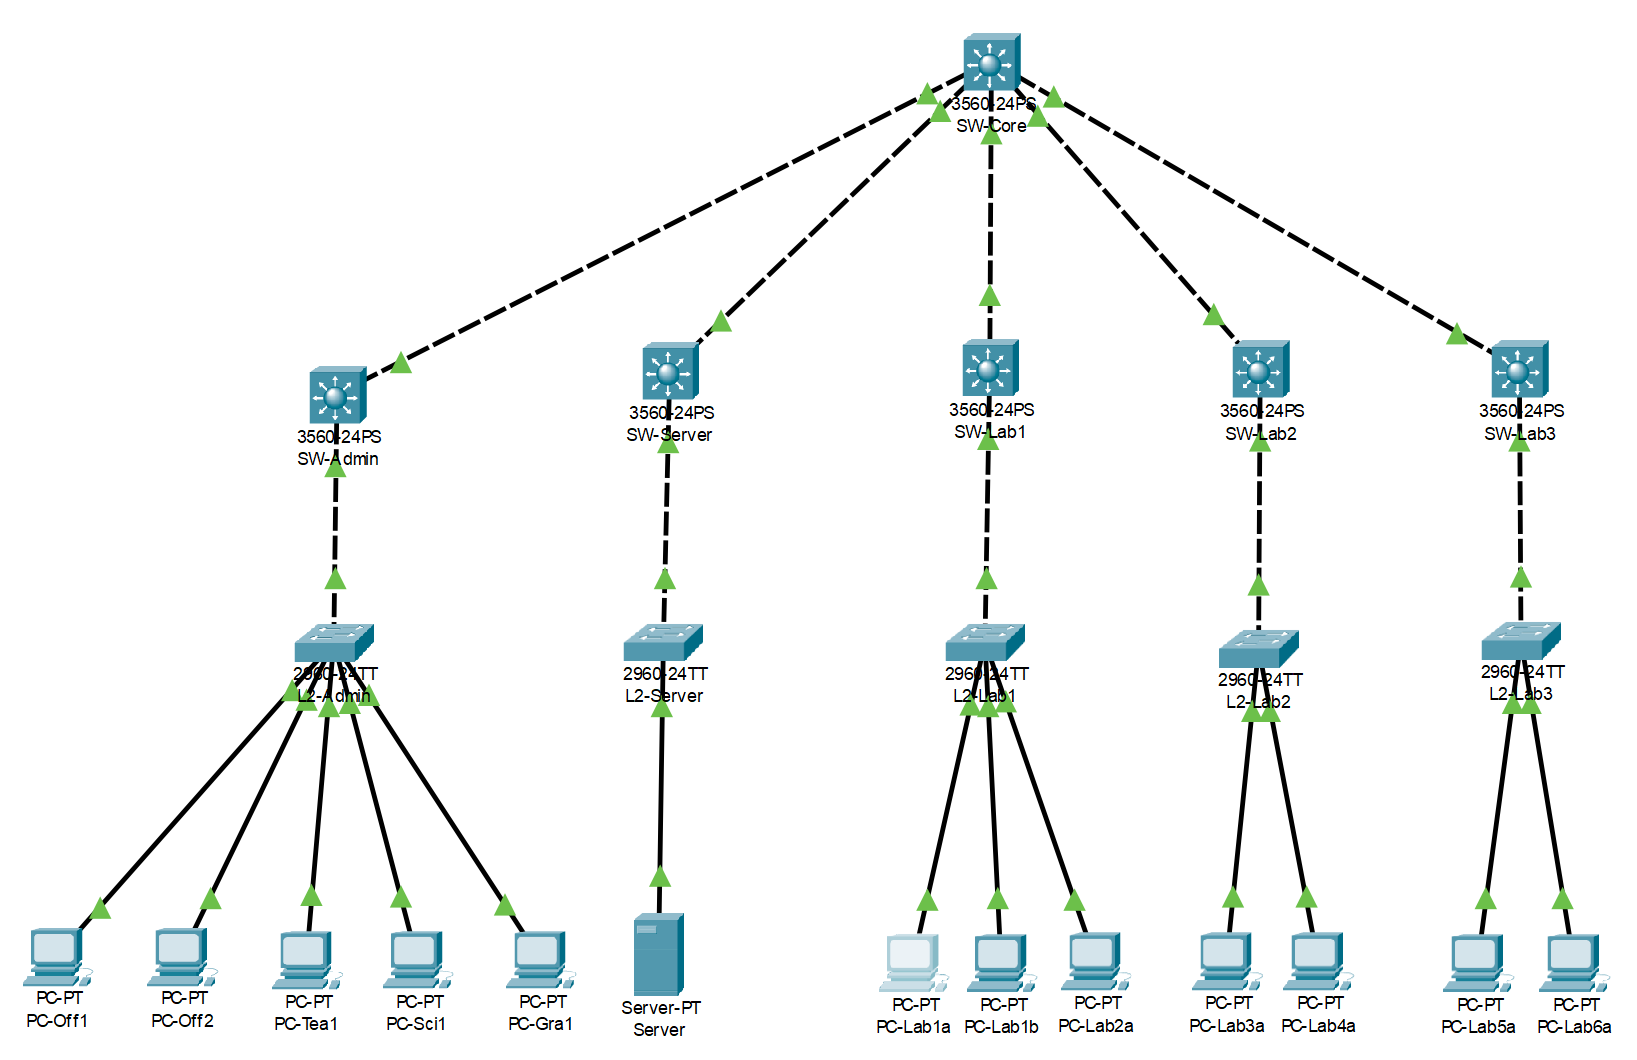
\includegraphics[width=0.95\textwidth]{fig1-topology.png}
\caption{Cisco Packet Tracer 完整拓扑图}
\label{fig:topo-pkt}
\end{figure}

\begin{notebox}
  \textbf{说明}：实际拓扑中每台三层交换机下方可挂接多台 24 口二层交换机，以覆盖相应区域的全部终端。上图为简化示意。
\end{notebox}

\textbf{层次说明：}

\begin{itemize}
  \item \textbf{核心层（Core）}：仅 SW-Core 一台，负责各汇聚交换机之间的路由转发，不直接连接终端；
  \item \textbf{汇聚层（Aggregation）}：SW-Server、SW-Admin、SW-Lab1、SW-Lab2、SW-Lab3 共 5 台，各自管理下属 VLAN 并将流量汇聚至核心层；
  \item \textbf{接入层（Access）}：24 口二层交换机，将各区域 PC 和服务器接入网络，按 VLAN 划分接入端口。
\end{itemize}

\subsection{IP 地址与 VLAN 规划}

\subsubsection*{个人计算机区域}

\begin{table}[H]
\centering
\caption{个人计算机区域 IP 地址与 VLAN 规划}
\label{tab:pc-ip}
\resizebox{\linewidth}{!}{%
\begin{tabular}{lclllclc}
\toprule
\textbf{用户群体} & \textbf{VLAN} & \textbf{网络地址} & \textbf{子网掩码} & \textbf{可用 IP 范围} & \textbf{主机数} & \textbf{默认网关} & \textbf{所属交换机} \\
\midrule
办公用    & 20  & 192.168.0.0   & 255.255.255.192 & .2 --- .61   & 60   & 192.168.0.1   & SW-Admin \\
教学用    & 30  & 192.168.0.64  & 255.255.255.192 & .66 --- .125 & 60   & 192.168.0.65  & SW-Admin \\
科研用    & 40  & 192.168.0.128 & 255.255.255.128 & .130 --- .249& 120  & 192.168.0.129 & SW-Admin \\
研究生    & 50  & 192.168.1.0   & 255.255.255.0   & .2 --- .201  & 200  & 192.168.1.1   & SW-Admin \\
学生实验室 1 & 60 & 192.168.2.0  & 255.255.255.0   & .2 --- .254  & $\leq$253 & 192.168.2.1   & SW-Lab1  \\
学生实验室 2 & 70 & 192.168.3.0  & 255.255.255.0   & .2 --- .254  & $\leq$253 & 192.168.3.1   & SW-Lab1  \\
学生实验室 3 & 80 & 192.168.4.0  & 255.255.255.0   & .2 --- .254  & $\leq$253 & 192.168.4.1   & SW-Lab2  \\
学生实验室 4 & 90 & 192.168.5.0  & 255.255.255.0   & .2 --- .254  & $\leq$253 & 192.168.5.1   & SW-Lab2  \\
学生实验室 5 & 100& 192.168.6.0  & 255.255.255.0   & .2 --- .254  & $\leq$253 & 192.168.6.1   & SW-Lab3  \\
学生实验室 6 & 110& 192.168.7.0  & 255.255.255.0   & .2 --- .254  & $\leq$253 & 192.168.7.1   & SW-Lab3  \\
\bottomrule
\end{tabular}
}

\smallskip
\footnotesize\textit{注：学生实验室 6 个网段共可容纳 6 × 253 = 1518 台主机，满足 1460 台学生实验电脑需求。}
\end{table}

\subsubsection*{服务器区域}

\begin{table}[H]
\centering
\caption{服务器区域 IP 地址与 VLAN 规划}
\label{tab:server-ip}
\resizebox{\linewidth}{!}{%
\begin{tabular}{lclllclc}
\toprule
\textbf{用途} & \textbf{VLAN} & \textbf{网络地址} & \textbf{子网掩码} & \textbf{可用 IP 范围} & \textbf{主机数} & \textbf{默认网关（已给定）} & \textbf{所属交换机} \\
\midrule
服务器区 & 10 & 172.16.1.0 & 255.255.255.192 & .1 --- .61 & 50 & 172.16.1.62 & SW-Server \\
\bottomrule
\end{tabular}
}

\smallskip
\footnotesize\textit{注：服务器区 /26 子网共 62 个可用地址（.1 --- .62），其中 .62 为网关，剩余 61 个地址供 50 台服务器使用，略有余量。}
\end{table}

\subsubsection*{三层交换机互联网段（/30 点对点链路）}

\begin{table}[H]
\centering
\caption{三层交换机互联网段}
\label{tab:interlink}
\begin{tabular}{llll}
\toprule
\textbf{链路} & \textbf{网络地址} & \textbf{SW-Core 侧 IP} & \textbf{对端 IP} \\
\midrule
SW-Core $\leftrightarrow$ SW-Server & 10.0.0.0/30  & 10.0.0.1  & 10.0.0.2  \\
SW-Core $\leftrightarrow$ SW-Admin  & 10.0.0.4/30  & 10.0.0.5  & 10.0.0.6  \\
SW-Core $\leftrightarrow$ SW-Lab1   & 10.0.0.8/30  & 10.0.0.9  & 10.0.0.10 \\
SW-Core $\leftrightarrow$ SW-Lab2   & 10.0.0.12/30 & 10.0.0.13 & 10.0.0.14 \\
SW-Core $\leftrightarrow$ SW-Lab3   & 10.0.0.16/30 & 10.0.0.17 & 10.0.0.18 \\
\bottomrule
\end{tabular}
\end{table}

\subsection{三层交换机路由设计}

采用\textbf{静态路由}方案，SW-Core 维护到各子网的明细路由，各汇聚交换机只需配置指向 SW-Core 的默认路由（0.0.0.0/0），结构简单、维护方便。

\subsubsection{静态路由汇总}

\textbf{SW-Core 需配置的路由条目：}

\begin{table}[H]
\centering
\caption{SW-Core 静态路由表}
\begin{tabular}{llll}
\toprule
\textbf{目标网络} & \textbf{掩码} & \textbf{下一跳} & \textbf{说明} \\
\midrule
172.16.1.0   & /26 & 10.0.0.2  & 服务器区 \\
192.168.0.0  & /26 & 10.0.0.6  & 办公区 \\
192.168.0.64 & /26 & 10.0.0.6  & 教学区 \\
192.168.0.128& /25 & 10.0.0.6  & 科研区 \\
192.168.1.0  & /24 & 10.0.0.6  & 研究生区 \\
192.168.2.0  & /24 & 10.0.0.10 & 学生实验室 1 \\
192.168.3.0  & /24 & 10.0.0.10 & 学生实验室 2 \\
192.168.4.0  & /24 & 10.0.0.14 & 学生实验室 3 \\
192.168.5.0  & /24 & 10.0.0.14 & 学生实验室 4 \\
192.168.6.0  & /24 & 10.0.0.18 & 学生实验室 5 \\
192.168.7.0  & /24 & 10.0.0.18 & 学生实验室 6 \\
\bottomrule
\end{tabular}
\end{table}

\textbf{各汇聚交换机}：统一配置默认路由指向 SW-Core 对应接口 IP。

\subsubsection{RIP 方案（备选）}

若需动态路由，可在所有三层交换机上启用 RIP v2：

\begin{codeblock}
router rip
 version 2
 no auto-summary
 network 10.0.0.0
 network 172.16.0.0
 network 192.168.0.0
 ! （根据各交换机实际网段添加）
\end{codeblock}

RIP v2 支持 VLSM（变长子网掩码），能自动学习并更新路由表，适合网络拓扑可能调整的场景。

% =========================================================
% 五、系统配置与实施
% =========================================================
\section{系统配置与实施}

本章给出完整的 Cisco Packet Tracer 仿真配置步骤。软件版本：\textbf{Cisco Packet Tracer 7.3.0}。

\subsection{Packet Tracer 拓扑搭建步骤}

\begin{enumerate}
  \item 打开 Packet Tracer，选择以下设备放置于工作区：
    \begin{itemize}
      \item \textbf{三层交换机}：\texttt{Cisco Catalyst 3560-24PS} × 6（命名为 SW-Core、SW-Server、SW-Admin、SW-Lab1、SW-Lab2、SW-Lab3）
      \item \textbf{二层交换机}：\texttt{Cisco Catalyst 2960-24TT} × 若干（每台三层交换机下方至少放 1 台）
      \item \textbf{服务器}：\texttt{Server-PT} × 1（代表服务器区，IP 设为 172.16.1.2）
      \item \textbf{PC}：\texttt{PC-PT} × 若干（每个 VLAN 至少放 2 台用于测试）
    \end{itemize}
  \item 用\textbf{铜制直通线（Copper Straight-Through）}连接：
    \begin{itemize}
      \item 三层交换机的 GigabitEthernet 口互联（SW-Core 的 Gi0/1 接 SW-Server 的 Gi0/1，以此类推）
      \item 三层交换机的 FastEthernet 口连接二层交换机
      \item 二层交换机的 FastEthernet 口连接 PC 和服务器
    \end{itemize}
\end{enumerate}

\subsection{终端设备 IP 配置}

在每台 PC 的 Desktop > IP Configuration 中，按照第四章规划表手动配置 IP 地址、子网掩码和默认网关。

\textbf{示例（办公区 PC，VLAN 20）：}

\begin{table}[H]
\centering
\caption{办公区 PC IP 配置示例（VLAN 20）}
\begin{tabular}{ll}
\toprule
\textbf{参数} & \textbf{值} \\
\midrule
IP Address     & 192.168.0.2 \\
Subnet Mask    & 255.255.255.192 \\
Default Gateway& 192.168.0.1 \\
\bottomrule
\end{tabular}
\end{table}

\textbf{服务器（VLAN 10）：}

\begin{table}[H]
\centering
\caption{服务器 IP 配置（VLAN 10）}
\begin{tabular}{ll}
\toprule
\textbf{参数} & \textbf{值} \\
\midrule
IP Address     & 172.16.1.2 \\
Subnet Mask    & 255.255.255.192 \\
Default Gateway& 172.16.1.62 \\
\bottomrule
\end{tabular}
\end{table}

\subsection{二层交换机配置}

每台二层交换机仅需创建相应 VLAN 并划分端口。以服务器区下方的二层交换机（L2-Server）为例：

\begin{codeblock}
! 进入配置模式
Switch>enable
Switch#configure terminal

! 重命名（可选）
Switch(config)#hostname L2-Server

! 创建 VLAN 10
L2-Server(config)#vlan 10
L2-Server(config-vlan)#exit

! 上联端口（连接 SW-Server）配置为 Trunk
L2-Server(config)#interface FastEthernet0/1
L2-Server(config-if)#switchport mode trunk
L2-Server(config-if)#exit

! 接入端口（连接服务器）配置为 Access，归属 VLAN 10
L2-Server(config)#interface range FastEthernet0/2-24
L2-Server(config-if-range)#switchport mode access
L2-Server(config-if-range)#switchport access vlan 10
L2-Server(config-if-range)#exit
L2-Server(config)#end
\end{codeblock}

其余各二层交换机按对应 VLAN ID 修改即可，方法完全相同。

\subsection{三层交换机 VLAN 配置及接口 IP 地址配置}

\subsubsection{SW-Core（核心交换机）}

\begin{codeblock}
SW-Core>enable
SW-Core#configure terminal
SW-Core(config)#hostname SW-Core

! 开启路由功能
SW-Core(config)#ip routing

! 配置连接 SW-Server 的路由口（Gi0/1 -> 10.0.0.1）
SW-Core(config)#interface GigabitEthernet0/1
SW-Core(config-if)#no switchport
SW-Core(config-if)#ip address 10.0.0.1 255.255.255.252
SW-Core(config-if)#no shutdown
SW-Core(config-if)#exit

! 配置连接 SW-Admin 的路由口（Gi0/2 -> 10.0.0.5）
SW-Core(config)#interface GigabitEthernet0/2
SW-Core(config-if)#no switchport
SW-Core(config-if)#ip address 10.0.0.5 255.255.255.252
SW-Core(config-if)#no shutdown
SW-Core(config-if)#exit

! 配置连接 SW-Lab1 的路由口（Fa0/1 -> 10.0.0.9）
SW-Core(config)#interface FastEthernet0/1
SW-Core(config-if)#no switchport
SW-Core(config-if)#ip address 10.0.0.9 255.255.255.252
SW-Core(config-if)#no shutdown
SW-Core(config-if)#exit

! 配置连接 SW-Lab2 的路由口（Fa0/2 -> 10.0.0.13）
SW-Core(config)#interface FastEthernet0/2
SW-Core(config-if)#no switchport
SW-Core(config-if)#ip address 10.0.0.13 255.255.255.252
SW-Core(config-if)#no shutdown
SW-Core(config-if)#exit

! 配置连接 SW-Lab3 的路由口（Fa0/3 -> 10.0.0.17）
SW-Core(config)#interface FastEthernet0/3
SW-Core(config-if)#no switchport
SW-Core(config-if)#ip address 10.0.0.17 255.255.255.252
SW-Core(config-if)#no shutdown
SW-Core(config-if)#exit

! 配置静态路由
SW-Core(config)#ip route 172.16.1.0 255.255.255.192 10.0.0.2
SW-Core(config)#ip route 192.168.0.0 255.255.255.192 10.0.0.6
SW-Core(config)#ip route 192.168.0.64 255.255.255.192 10.0.0.6
SW-Core(config)#ip route 192.168.0.128 255.255.255.128 10.0.0.6
SW-Core(config)#ip route 192.168.1.0 255.255.255.0 10.0.0.6
SW-Core(config)#ip route 192.168.2.0 255.255.255.0 10.0.0.10
SW-Core(config)#ip route 192.168.3.0 255.255.255.0 10.0.0.10
SW-Core(config)#ip route 192.168.4.0 255.255.255.0 10.0.0.14
SW-Core(config)#ip route 192.168.5.0 255.255.255.0 10.0.0.14
SW-Core(config)#ip route 192.168.6.0 255.255.255.0 10.0.0.18
SW-Core(config)#ip route 192.168.7.0 255.255.255.0 10.0.0.18

SW-Core(config)#end
\end{codeblock}

\subsubsection{SW-Server（服务器汇聚交换机）}

\begin{codeblock}
SW-Server>enable
SW-Server#configure terminal
SW-Server(config)#hostname SW-Server
SW-Server(config)#ip routing

! 创建 VLAN 10
SW-Server(config)#vlan 10
SW-Server(config-vlan)#exit

! VLAN 10 SVI 接口（服务器区网关，已给定 172.16.1.62）
SW-Server(config)#interface vlan 10
SW-Server(config-if)#ip address 172.16.1.62 255.255.255.192
SW-Server(config-if)#no shutdown
SW-Server(config-if)#exit

! 上联路由口（连接 SW-Core Gi0/1）
SW-Server(config)#interface GigabitEthernet0/1
SW-Server(config-if)#no switchport
SW-Server(config-if)#ip address 10.0.0.2 255.255.255.252
SW-Server(config-if)#no shutdown
SW-Server(config-if)#exit

! 下联口连接 L2-Server，设为 Trunk
SW-Server(config)#interface FastEthernet0/1
SW-Server(config-if)#switchport trunk encapsulation dot1q
SW-Server(config-if)#switchport mode trunk
SW-Server(config-if)#exit

! 默认路由指向 SW-Core
SW-Server(config)#ip route 0.0.0.0 0.0.0.0 10.0.0.1
SW-Server(config)#end
\end{codeblock}

\subsubsection{SW-Admin（办公/教学/科研/研究生汇聚交换机）}

\begin{codeblock}
SW-Admin>enable
SW-Admin#configure terminal
SW-Admin(config)#hostname SW-Admin
SW-Admin(config)#ip routing

! 创建 VLAN
SW-Admin(config)#vlan 20
SW-Admin(config-vlan)#vlan 30
SW-Admin(config-vlan)#vlan 40
SW-Admin(config-vlan)#vlan 50
SW-Admin(config-vlan)#exit

! VLAN SVI 接口（各 VLAN 网关）
SW-Admin(config)#interface vlan 20
SW-Admin(config-if)#ip address 192.168.0.1 255.255.255.192
SW-Admin(config-if)#no shutdown
SW-Admin(config-if)#exit

SW-Admin(config)#interface vlan 30
SW-Admin(config-if)#ip address 192.168.0.65 255.255.255.192
SW-Admin(config-if)#no shutdown
SW-Admin(config-if)#exit

SW-Admin(config)#interface vlan 40
SW-Admin(config-if)#ip address 192.168.0.129 255.255.255.128
SW-Admin(config-if)#no shutdown
SW-Admin(config-if)#exit

SW-Admin(config)#interface vlan 50
SW-Admin(config-if)#ip address 192.168.1.1 255.255.255.0
SW-Admin(config-if)#no shutdown
SW-Admin(config-if)#exit

! 上联路由口（连接 SW-Core Gi0/2）
SW-Admin(config)#interface GigabitEthernet0/1
SW-Admin(config-if)#no switchport
SW-Admin(config-if)#ip address 10.0.0.6 255.255.255.252
SW-Admin(config-if)#no shutdown
SW-Admin(config-if)#exit

! 下联口连接 L2-Admin，设为 Trunk
SW-Admin(config)#interface FastEthernet0/1
SW-Admin(config-if)#switchport trunk encapsulation dot1q
SW-Admin(config-if)#switchport mode trunk
SW-Admin(config-if)#exit

! 默认路由指向 SW-Core
SW-Admin(config)#ip route 0.0.0.0 0.0.0.0 10.0.0.5
SW-Admin(config)#end
\end{codeblock}

\subsubsection{SW-Lab1（学生实验室 1、2 汇聚交换机）}

\begin{codeblock}
SW-Lab1>enable
SW-Lab1#configure terminal
SW-Lab1(config)#hostname SW-Lab1
SW-Lab1(config)#ip routing

SW-Lab1(config)#vlan 60
SW-Lab1(config-vlan)#vlan 70
SW-Lab1(config-vlan)#exit

SW-Lab1(config)#interface vlan 60
SW-Lab1(config-if)#ip address 192.168.2.1 255.255.255.0
SW-Lab1(config-if)#no shutdown
SW-Lab1(config-if)#exit

SW-Lab1(config)#interface vlan 70
SW-Lab1(config-if)#ip address 192.168.3.1 255.255.255.0
SW-Lab1(config-if)#no shutdown
SW-Lab1(config-if)#exit

SW-Lab1(config)#interface FastEthernet0/1
SW-Lab1(config-if)#no switchport
SW-Lab1(config-if)#ip address 10.0.0.10 255.255.255.252
SW-Lab1(config-if)#no shutdown
SW-Lab1(config-if)#exit

! 下联 Trunk 口
SW-Lab1(config)#interface FastEthernet0/2
SW-Lab1(config-if)#switchport trunk encapsulation dot1q
SW-Lab1(config-if)#switchport mode trunk
SW-Lab1(config-if)#exit

SW-Lab1(config)#ip route 0.0.0.0 0.0.0.0 10.0.0.9
SW-Lab1(config)#end
\end{codeblock}

\subsubsection{SW-Lab2（学生实验室 3、4 汇聚交换机）}

\begin{codeblock}
SW-Lab2>enable
SW-Lab2#configure terminal
SW-Lab2(config)#hostname SW-Lab2
SW-Lab2(config)#ip routing

SW-Lab2(config)#vlan 80
SW-Lab2(config-vlan)#vlan 90
SW-Lab2(config-vlan)#exit

SW-Lab2(config)#interface vlan 80
SW-Lab2(config-if)#ip address 192.168.4.1 255.255.255.0
SW-Lab2(config-if)#no shutdown
SW-Lab2(config-if)#exit

SW-Lab2(config)#interface vlan 90
SW-Lab2(config-if)#ip address 192.168.5.1 255.255.255.0
SW-Lab2(config-if)#no shutdown
SW-Lab2(config-if)#exit

SW-Lab2(config)#interface FastEthernet0/1
SW-Lab2(config-if)#no switchport
SW-Lab2(config-if)#ip address 10.0.0.14 255.255.255.252
SW-Lab2(config-if)#no shutdown
SW-Lab2(config-if)#exit

SW-Lab2(config)#interface FastEthernet0/2
SW-Lab2(config-if)#switchport trunk encapsulation dot1q
SW-Lab2(config-if)#switchport mode trunk
SW-Lab2(config-if)#exit

SW-Lab2(config)#ip route 0.0.0.0 0.0.0.0 10.0.0.13
SW-Lab2(config)#end
\end{codeblock}

\subsubsection{SW-Lab3（学生实验室 5、6 汇聚交换机）}

\begin{codeblock}
SW-Lab3>enable
SW-Lab3#configure terminal
SW-Lab3(config)#hostname SW-Lab3
SW-Lab3(config)#ip routing

SW-Lab3(config)#vlan 100
SW-Lab3(config-vlan)#vlan 110
SW-Lab3(config-vlan)#exit

SW-Lab3(config)#interface vlan 100
SW-Lab3(config-if)#ip address 192.168.6.1 255.255.255.0
SW-Lab3(config-if)#no shutdown
SW-Lab3(config-if)#exit

SW-Lab3(config)#interface vlan 110
SW-Lab3(config-if)#ip address 192.168.7.1 255.255.255.0
SW-Lab3(config-if)#no shutdown
SW-Lab3(config-if)#exit

SW-Lab3(config)#interface FastEthernet0/1
SW-Lab3(config-if)#no switchport
SW-Lab3(config-if)#ip address 10.0.0.18 255.255.255.252
SW-Lab3(config-if)#no shutdown
SW-Lab3(config-if)#exit

SW-Lab3(config)#interface FastEthernet0/2
SW-Lab3(config-if)#switchport trunk encapsulation dot1q
SW-Lab3(config-if)#switchport mode trunk
SW-Lab3(config-if)#exit

SW-Lab3(config)#ip route 0.0.0.0 0.0.0.0 10.0.0.17
SW-Lab3(config)#end
\end{codeblock}

\subsection{学院网站设计}

\subsubsection{功能版块及初步描述}

学院官方网站共设计 \textbf{5 个功能模块}，满足师生的信息获取与交互需求：

\begin{table}[H]
\centering
\caption{学院官方网站功能模块}
\begin{tabular}{L{2cm}L{2.5cm}L{8.5cm}}
\toprule
\textbf{模块名称} & \textbf{主要功能} & \textbf{初步描述} \\
\midrule
\textbf{首页}     & 学院形象展示 & 展示学院名称、学院简介、最新公告和快速导航入口；页面简洁大方，体现学院文化氛围 \\
\midrule
\textbf{教学平台} & 教学资源汇聚 & 发布课程信息、教学大纲、课件下载链接；涵盖本科生与研究生课程，支持分类检索 \\
\midrule
\textbf{科研成果} & 科研信息展示 & 展示科研项目立项情况、学术论文、专利成果；设置研究生成果专栏，激励学术创新 \\
\midrule
\textbf{新闻动态} & 校园资讯中心 & 发布学院新闻、活动通知、招聘信息、竞赛动态；按时间倒序排列，支持分类浏览 \\
\midrule
\textbf{联系我们} & 信息与反馈   & 展示学院地址、联系电话、电子邮箱；提供在线留言功能，方便外部机构与学院沟通 \\
\bottomrule
\end{tabular}
\end{table}

\subsubsection{Packet Tracer 中配置 HTTP 服务}

\begin{enumerate}
  \item 点击服务器（IP 172.16.1.2），进入 \textbf{Services > HTTP}；
  \item 将 HTTP 服务设置为 \textbf{On}；
  \item 点击 \textbf{index.html}，粘贴以下 HTML 代码；
  \item 保存后，各 PC 可在 Desktop > Web Browser 中输入 \texttt{http://172.16.1.2} 访问学院主页。
\end{enumerate}

\textbf{index.html 源代码：}

\begin{htmlblock}
<!DOCTYPE html>
<html lang="zh-CN">
<head>
  <meta charset="UTF-8">
  <title>某信息工程学院</title>
  <style>
    body { margin:0; font-family:Arial,sans-serif; background:#f0f4f8; }
    header { background:#1a5fa8; color:#fff; padding:24px 40px; }
    header h1 { margin:0; font-size:28px; }
    header p  { margin:4px 0 0; font-size:14px; opacity:0.85; }
    nav { background:#154d8a; display:flex; padding:0 40px; }
    nav a { color:#fff; text-decoration:none; padding:12px 20px;
            font-size:15px; display:block; }
    nav a:hover { background:#1a6ec7; }
    .main { max-width:960px; margin:30px auto; padding:0 20px; }
    .card { background:#fff; border-radius:6px; padding:24px;
            margin-bottom:20px; box-shadow:0 2px 6px rgba(0,0,0,.08); }
    .card h2 { margin-top:0; color:#1a5fa8; font-size:20px; }
    ul { padding-left:20px; line-height:1.9; }
    .grid { display:flex; gap:20px; flex-wrap:wrap; }
    .grid .card { flex:1; min-width:260px; }
    footer { background:#1a5fa8; color:#fff; text-align:center;
             padding:16px; font-size:13px; }
  </style>
</head>
<body>
<header>
  <h1>某信息工程学院</h1>
  <p>教学 · 科研 · 创新 · 服务</p>
</header>
<nav>
  <a href="index.html">首页</a>
  <a href="teaching.html">教学平台</a>
  <a href="research.html">科研成果</a>
  <a href="news.html">新闻动态</a>
  <a href="contact.html">联系我们</a>
</nav>
<div class="main">
  <div class="card">
    <h2>学院简介</h2>
    <p>某信息工程学院成立于20世纪末，下设计算机科学系、网络工程系和信息安全系，
    现有教职工180余名，全日制在校学生近2000名，致力于培养具有扎实理论基础和
    较强工程实践能力的高素质信息技术人才。</p>
  </div>
  <div class="grid">
    <div class="card">
      <h2>最新公告</h2>
      <ul>
        <li>2024年秋季学期选课通知</li>
        <li>第十届科技创新大赛报名开始</li>
        <li>实验中心暑期开放安排</li>
        <li>研究生学位论文答辩名单公示</li>
      </ul>
    </div>
    <div class="card">
      <h2>快速导航</h2>
      <ul>
        <li><a href="teaching.html">课程资源下载</a></li>
        <li><a href="research.html">学术论文查询</a></li>
        <li><a href="news.html">校园活动报名</a></li>
        <li><a href="contact.html">在线留言反馈</a></li>
      </ul>
    </div>
  </div>
</div>
<footer>
  &copy; 2024 某信息工程学院 版权所有 &nbsp;|&nbsp; 地址：XX市XX路XX号
</footer>
</body>
</html>
\end{htmlblock}

\textbf{teaching.html 核心内容：}

\begin{htmlblock}
<!DOCTYPE html>
<html lang="zh-CN">
<head>
  <meta charset="UTF-8">
  <title>教学平台 - 某信息工程学院</title>
  <style>
    body{margin:0;font-family:Arial,sans-serif;background:#f0f4f8;}
    header{background:#1a5fa8;color:#fff;padding:24px 40px;}
    nav{background:#154d8a;display:flex;padding:0 40px;}
    nav a{color:#fff;text-decoration:none;padding:12px 20px;font-size:15px;}
    nav a:hover{background:#1a6ec7;}
    .main{max-width:960px;margin:30px auto;padding:0 20px;}
    .card{background:#fff;border-radius:6px;padding:24px;margin-bottom:20px;
          box-shadow:0 2px 6px rgba(0,0,0,.08);}
    .card h2{margin-top:0;color:#1a5fa8;}
    table{width:100%;border-collapse:collapse;margin-top:12px;}
    th,td{padding:10px 14px;border:1px solid #ddd;text-align:left;}
    th{background:#1a5fa8;color:#fff;}
    footer{background:#1a5fa8;color:#fff;text-align:center;
           padding:16px;font-size:13px;}
  </style>
</head>
<body>
<header><h1>教学平台</h1></header>
<nav>
  <a href="index.html">首页</a><a href="teaching.html">教学平台</a>
  <a href="research.html">科研成果</a><a href="news.html">新闻动态</a>
  <a href="contact.html">联系我们</a>
</nav>
<div class="main">
  <div class="card">
    <h2>本科生课程</h2>
    <table>
      <tr><th>课程名称</th><th>学分</th><th>开课学期</th><th>课件下载</th></tr>
      <tr><td>计算机网络</td><td>3</td><td>大三上</td><td>待更新</td></tr>
      <tr><td>操作系统</td><td>4</td><td>大二下</td><td>待更新</td></tr>
      <tr><td>数据结构</td><td>3</td><td>大二上</td><td>待更新</td></tr>
    </table>
  </div>
  <div class="card">
    <h2>研究生课程</h2>
    <table>
      <tr><th>课程名称</th><th>学分</th><th>开课学期</th><th>课件下载</th></tr>
      <tr><td>高级计算机网络</td><td>3</td><td>研一上</td><td>待更新</td></tr>
      <tr><td>机器学习</td><td>3</td><td>研一上</td><td>待更新</td></tr>
    </table>
  </div>
</div>
<footer>&copy; 2024 某信息工程学院</footer>
</body>
</html>
\end{htmlblock}

\subsection{Cisco Packet Tracer 仿真验证}

配置完成后，按以下步骤验证网络功能：

\subsubsection{验证一：同一 VLAN 内互通}

在 VLAN 20（办公区）中，从 PC1（192.168.0.2）ping PC2（192.168.0.3）：

\begin{codeblock}
PC1> ping 192.168.0.3
Reply from 192.168.0.3: bytes=32 time<1ms TTL=128
\end{codeblock}

\textbf{预期结果}：ping 通，说明同 VLAN 内二层通信正常。

\begin{figure}[H]
\centering
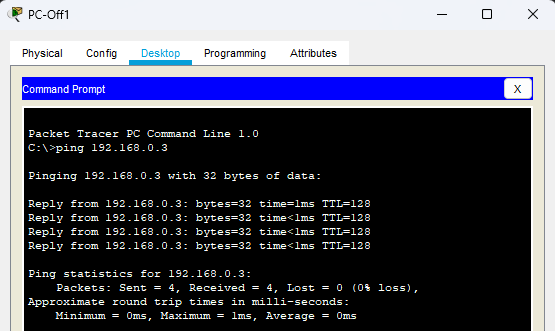
\includegraphics[width=0.85\textwidth]{fig2-test1.png}
\caption{同一 VLAN 内 PC 互 ping 测试}
\label{fig:test1}
\end{figure}

\subsubsection{验证二：跨 VLAN 互通}

从 VLAN 20 的 PC1（192.168.0.2）ping VLAN 60 的学生机（192.168.2.2）：

\begin{codeblock}
PC1> ping 192.168.2.2
Reply from 192.168.2.2: bytes=32 time<1ms TTL=126
\end{codeblock}

\textbf{预期结果}：ping 通（经过 SW-Admin → SW-Core → SW-Lab1 路由），TTL 为 126（每经过一台三层设备减 1）。

\begin{figure}[H]
\centering
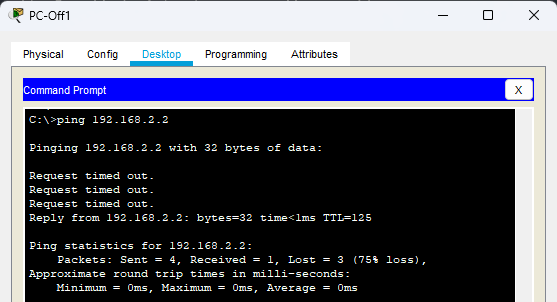
\includegraphics[width=0.85\textwidth]{fig3-test2.png}
\caption{跨 VLAN 通信测试（VLAN 20 ping VLAN 60）}
\label{fig:test2}
\end{figure}

\subsubsection{验证三：访问服务器区}

从 VLAN 60 的学生机（192.168.2.2）ping 服务器（172.16.1.2）：

\begin{codeblock}
StudentPC> ping 172.16.1.2
Reply from 172.16.1.2: bytes=32 time<1ms TTL=125
\end{codeblock}

\textbf{预期结果}：ping 通，三层路由正确。

\begin{figure}[H]
\centering
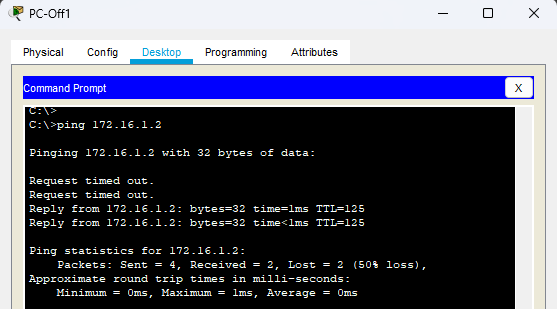
\includegraphics[width=0.85\textwidth]{fig4-test3.png}
\caption{PC ping 服务器 172.16.1.2}
\label{fig:test3}
\end{figure}

\subsubsection{验证四：访问学院网站}

在任意 PC 的 Desktop > Web Browser 中输入 \texttt{http://172.16.1.2}，应显示学院官方主页 HTML 内容。

\begin{figure}[H]
\centering
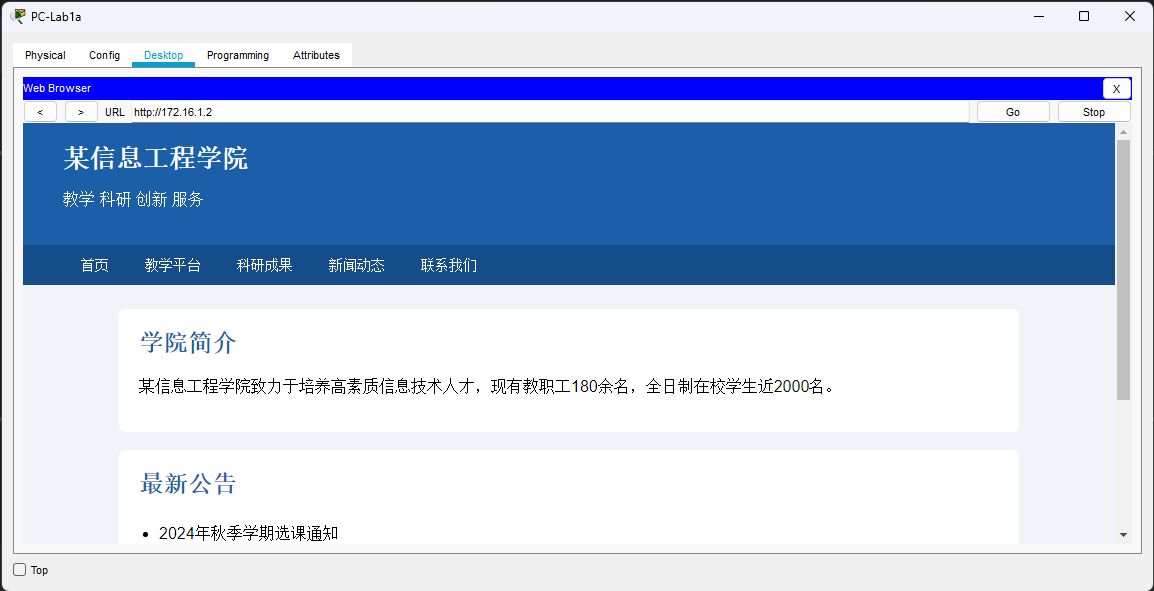
\includegraphics[width=0.85\textwidth]{fig5-test4.png}
\caption{PC 浏览器访问学院官方网站}
\label{fig:test4}
\end{figure}

\subsubsection{验证五：学生区访问服务器}

从 VLAN 60 的学生机（192.168.2.2）ping 服务器（172.16.1.2），验证学生区与服务器区的跨网段互通。

\textbf{预期结果}：ping 通，说明全网路由配置正确，各用户区均可访问服务器区。

\begin{figure}[H]
\centering
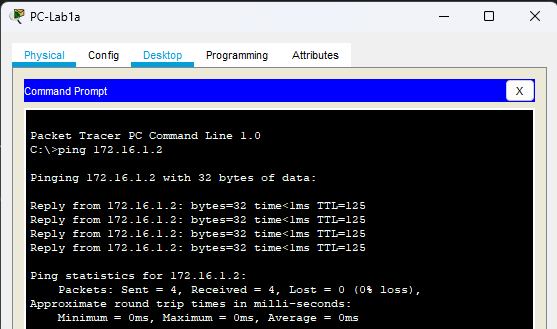
\includegraphics[width=0.85\textwidth]{fig6-test5.png}
\caption{学生区 PC ping 服务器 172.16.1.2}
\label{fig:test5}
\end{figure}

% =========================================================
% 六、工程预算与进度安排
% =========================================================
\section{工程预算与进度安排}

\subsection{工程预算}

\begin{notebox}
  注：PC 已采购，预算仅计算网络设备及布线材料。
\end{notebox}

\begin{table}[H]
\centering
\caption{工程预算明细}
\begin{tabular}{L{5.5cm}C{2cm}C{2cm}C{2.5cm}}
\toprule
\textbf{项目} & \textbf{单价（元）} & \textbf{数量} & \textbf{小计（元）} \\
\midrule
Cisco Catalyst 3560-24PS 三层交换机 & 3\,800 & 6 台  & 22\,800 \\
Cisco Catalyst 2960-24TT 二层交换机 & 900   & 20 台 & 18\,000 \\
Cat5e 超五类双绞线（箱，305 m/箱）  & 280   & 10 箱 & 2\,800  \\
RJ-45 水晶头（100 个/包）           & 25    & 20 包 & 500     \\
千兆多模光纤跳线                    & 80    & 10 条 & 800     \\
PVC 线管及配件                      & ---   & ---   & 2\,000  \\
配线架及机柜                        & 1\,200 & 3 套 & 3\,600  \\
安装调试人工费                      & ---   & ---   & 8\,000  \\
系统测试与验收费                    & ---   & ---   & 3\,000  \\
\midrule
\textbf{合计}                       & & & \textbf{61\,500} \\
不可预见费（约 10\%）               & & & 6\,150  \\
\midrule
\textbf{总计}                       & & & \textbf{$\approx$ 67\,650} \\
\bottomrule
\end{tabular}
\end{table}

\subsection{进度安排}

\begin{table}[H]
\centering
\caption{项目进度安排}
\begin{tabular}{L{3.5cm}L{8cm}C{2cm}}
\toprule
\textbf{阶段} & \textbf{工作内容} & \textbf{计划天数} \\
\midrule
第 1～2 天  & 需求调研、方案讨论、可行性分析               & 2 天 \\
第 3～4 天  & IP 地址规划、VLAN 设计、拓扑设计             & 2 天 \\
第 5～6 天  & 设备采购及到货验收                           & 2 天 \\
第 7～9 天  & 综合布线（穿管、敷线、打线、测试）           & 3 天 \\
第 10～12 天& 交换机安装上架、VLAN 配置、路由配置          & 3 天 \\
第 13 天    & 服务器配置、网站部署                         & 1 天 \\
第 14 天    & 全网联通性测试与问题整改                     & 1 天 \\
第 15 天    & 竣工验收、文档整理、用户培训                 & 1 天 \\
\midrule
\textbf{合计} & & \textbf{15 天} \\
\bottomrule
\end{tabular}
\end{table}

% =========================================================
% 七、实验总结
% =========================================================
\section{实验总结}

本次课程设计选择题目三，以某学院为背景，完成了一套完整的校园局域网规划方案。主要收获与体会如下：

\textbf{IP 地址规划的严谨性：}学院分配的地址空间（192.168.0.0---192.168.7.255）总量固定，需根据各用户群体的实际规模合理选取子网掩码。办公和教学群体规模较小（60 台），选用 /26 子网（62 个可用地址）恰好合适；科研群体 120 台，选用 /25 子网；研究生和学生群体采用 /24 子网。精确的子网划分既避免了地址浪费，又为未来少量扩展保留了余量。

\textbf{三层交换机的合理分工：}6 台三层交换机在核心层—汇聚层架构下各司其职，SW-Core 专注路由汇聚，其余 5 台专注各自区域的 VLAN 管理和网关功能，职责清晰、结构合理。

\textbf{静态路由的可行性：}在网络规模和拓扑固定的校园网环境中，静态路由配置简单、无协议开销，完全可以满足需求。实验中通过在 SW-Core 上配置 11 条静态路由，实现了全网互通。

\textbf{Cisco Packet Tracer 的实践价值：}仿真工具让网络设计"看得见、摸得着"。通过 ping 测试和 Web 访问验证，直观地确认了 VLAN 隔离和跨 VLAN 路由的正确性，也加深了对三层交换工作原理的理解。

通过本次课程设计，综合运用了计算机网络课程中 VLAN、子网划分、三层路由等核心知识，将理论与实践有机结合，为今后从事网络规划与管理工作打下了良好基础。

% =========================================================
% 八、参考文献
% =========================================================
\section*{参考文献}
\addcontentsline{toc}{section}{参考文献}

\begin{enumerate}[label={[\arabic*]}]
  \item 谢希仁. 计算机网络（第 8 版）[M]. 电子工业出版社，2022.
  \item Cisco Systems. Cisco Catalyst 3560 Series Switches Data Sheet [EB/OL]. \url{https://www.cisco.com}
  \item Cisco Systems. Cisco Catalyst 2960 Series Switches Data Sheet [EB/OL]. \url{https://www.cisco.com}
  \item Cisco Systems. IP Routing on Cisco IOS [EB/OL]. \url{https://www.cisco.com/c/zh_cn/tech/ip/ip-routing/index.html}
  \item Packet Tracer Official Tutorials [EB/OL]. \url{https://tutorials.ptnetacad.net/}
  \item 孙学聪, 杨进才. 计算机网络实验教程[M]. 清华大学出版社，2017.
\end{enumerate}

\end{document}
